\chapter{Planificación}
\label{sec:plani}
En este capítulo detallaré todo lo relativo a la planificación, cuantificación de recursos y
estimación del proyecto. 

\section{Metodología utilizada}
\label{sec:meto}
Desde que se empiezan a programar los primeros ordenadores en la historia, la programación
siempre ha sido minguneada y considerada bastante lejos de una actividad científica. Todo
empezó a cambiar cuando los scripts permitían realizar cálculos como ninguna otra
herramienta hasta el momento. Fue la matemática Margaret Hamilton quien planteó por
primera vez que los sistemas informáticos tenían que integrar tres componentes: hardware,
software y los usuarios que los iban a usar. Fue Margaret Hamiltonen, cuando se produce lo
que conocemos como crisis del software en 1968 quien acuñó en la \textit{NATO Software
Engineering Conference} el termino \textbf{Ingeniería} al proceso de creación de software. En ese
momento donde parecía que crear software duradero y escalable en el tiempo era misión
imposible hizo que se invirtiera en investigación y se construyera conocimiento. Este
conocimiento es lo que hoy llamamos Ingeniería de Software: herramientas, técnicas de
especificación y diseño que nos permiten especificar, desarrollar, validar y evolucionar
como en cualquier otra disciplina ingenieril.

Las desarrollo ágiles presentan una forma distinta de trabajar y organizarse, adaptándose
a las condiciones cambiantes que puedan surgir, aprovechando estos cambios para obtener
ventajas. Con este tipo de metodologías podemos dividir el trabajo en pequeñas piezas de
manera que podemos ir realizándolos de forma iterativa añadiendo valor concreto al
producto en cada iteración.

Se ha barajado utilizar una de las dos metodologías más empleadas en la industria: Scrum y
eXtreme Programming. eXtreme programming ha sido descartada por la imposibilidad de
aplicación en términos de tiempo y recursos humanos. Los roles y artefactos exigidos por
esta metodología son indiscutiblemente para un equipo de desarrollo segmentado. Sin
embargo y en comparación con Scrum es una metodología muy enfocada en el proceso de
desarrollo. Obliga a desarrollar guiándose de pruebas, a programar en parejas y asegurar
la calidad del código en todas las etapas.

Scrum en cambio se muestra más flexible. En el año 2001 que K. Schwaber y Mike Beedle
publican el primer libro sobre Scrum \cite{agile_book}: Agile Software Development with
Scrum esta metodología se ha convertido en la más utilizada para el desarrollo de
software. Siendo precisos y prudentes tampoco es posible aplicar propiamente dicho Scrum
en este proyecto\ldots fundamentalmente por ser una persona a cargo de todo el proceso.

Por tanto, me he permitido crear mi propia metodología de desarrollo basándome en los tres
valores fundamentales que ofrecen estas tecnologías:
\begin{itemize}
    \item \textbf{Transparencia}: en todo momento se ha de conocer en qué se está
    trabajando, que problemas se está teniendo y/o si existe algún bloqueo asociado.
    \item \textbf{Inspección}: se ha de inspeccionar y no perder de vista el progreso para
    conseguir el objetivo. La trazabilidad del trabajo nos la ofrece el SCV \footnote{source
    control versioning} en nuestro caso git en GitHub con incorporación de funcionalidad por pull
    request.
    \item \textbf{Adaptación}: poder reaccionar a tiempo a los cambios requeridos por los
    stakeholders.
\end{itemize}


\section{Herramientas}
En esta sección voy a comentar las herramientas utilizadas para cumplir con los objetivos
metodológicos marcados en el anterior capítulo.

Para el contribuir con la segunda característica introspectiva citada anteriormente,
necesitamos no perder de vista el progreso para conseguir el objetivo. Se ha recurrido a
utilizar un sistema de control de versiones, sin discusión alguna GIT ha sido la
herramienta seleccionada. Se hace necesaria una forja donde respaldar nuestro código,
GitHub ha sido la opción seleccionada para alojar el código debido a lo ampliamente
utilizada que es la plataforma y las características premium que nos ofrece una cuenta universitaria como los
tableros Kanban, integración continua con GitHub Actions\ldots

Haciendo uso de esta herramienta, se han definido unas serie de milestones que agrupan
historias de usuario e \textit{issues} o tareas a realizar. Los incrementos en el trabajo se han
ido realizando por medio de \textit{Pull Request} y cada una de estas lleva enlazada una o varias
issues. Se puede ver el panel de issues en \ref{fig:issues-HU}.

\subsection{Milestones}
Los milestones hacen referencia al conjunto de productos mínimamente viables que se van
generando conforme se avanza en el desarrollo del proyecto. Un milestone está formado por
un conjunto de issues, se entiende finalizado un milestone cuando se han contemplado todos
los issues asociados. Los milestones creados se pueden observar en el repositorio de
GitHub y son los siguientes:
\begin{enumerate}
    \item \textbf{Infraestructura}: Puesta en marcha de la integración continua, creación
    de las primeras historias de usuario y tareas.
    \item \textbf{Modelo de datos}: definición de las clases que conforman el dominio del
    problema, atendiendo al estado del arte y primeras excepciones. 
    \item \textbf{Predicción y gráficos}: podemos comenzar a trabajar con el modelo de
    datos para realizar someras predicciones sobre los datos y obtener gráficas derivadas
    de la agrupación de éstos. He denominado \textit{managers} a la lógica software que
    realiza esta funcionalidad.
    \item \textbf{Acceso a recursos y a los managers}: supone la interfaz de comunicación
    agnóstica con la que podemos acceder a los datos y realizar las operaciones descritas
    en el milestone anterior de forma agnóstica utilizando el protocolo REST que pueda ser
    utilizada por otros desarrolladores para construir aplicaciones con distintos
    objetivos.
    \item \textbf{Sistema avanzado de consultas}: implementación del lenguaje de consulta
    y manipulación de datos para API GraphQL que permita consumir la API satisfaciendo las
    necesidades de los usuarios ficticios.
\end{enumerate}

Todas las etapas han incluido los pertinentes de los capítulos de la memoria y el pretexto
a las decisiones técnicas elegidas para implementar la solución.


\subsection{Historias de usuario}
\label{sec:hu2}
Como estamos trabajando con una metodología de desarrollo ágil tenemos que expresar las
necesidades reales de los usuarios desde sus puntos de vista para lograr la
interacción del equipo de desarrollo con el usuario. Ello se consigue por medio de
historias de usuario, en adelante HU. Las HUs tienen que cumplir una serie de condiciones \cite{dddjj}:
\begin{itemize}
    \item Se tiene que identificar para que usuario se va a desarrollar la historia.
    \item La HU siempre está en el dominio del problema y siempre es narrada desde el
    punto de vista de ese usuario. Tiene que expresar el beneficio que obtendrá dicho
    usuario cuando se haya implementado la HU.
    \item La HU mayormente requiere la programación de cierta lógica de negocio. 
\end{itemize}
Todo lo que no cumpla estas características no son más que tareas enmarcadas en el proceso
de desarrollo. De las siguientes historias de usuarios se han generarán tareas específicas
cuya realización avanza en la HU.
\begin{itemize}
    \item \textbf{Como tribunal tengo que poder leer de forma ordenada y estructurada la
    memoria.} 
    Se enmarca en la naturaleza que tiene este trabajo de ser presentado y
    evaluado como TFG. Cuyo criterio de aceptación es: la elaboración de una memoria
    estructurada, detallada y ordenada que facilite el entendimiento del trabajo.

    \item \textbf{Trabajar con los datos de mortandad.}
    Como usuario programadora
    quiero poder acceder para trabajar a los datos de mortandad
    tal que pueda construir aplicaciones y servicios sin tener que preocuparme de montar cualquier infraestructura para obtener estos datos.

    \item \textbf{Predicciones y gráficos basados en los datos.}
    Como programadora quiero poder obtener predicciones sobre el incremento de defunciones
    tal que dada una enfermedad pueda obtener su predicción de defunciones en los próximos años.
\end{itemize}

Estas historias de usuarios que expresan una funcionalidad a alcanzar son ejecutadas
mediante tareas que en su completitud satisfacen el deseo del usuario. Se pueden observar en
el \href{https://github.com/pablojjimenez/TFG/issues}{tablero de issues} de GitHub.

\FloatBarrier
\begin{figure}[h]
	\centering
	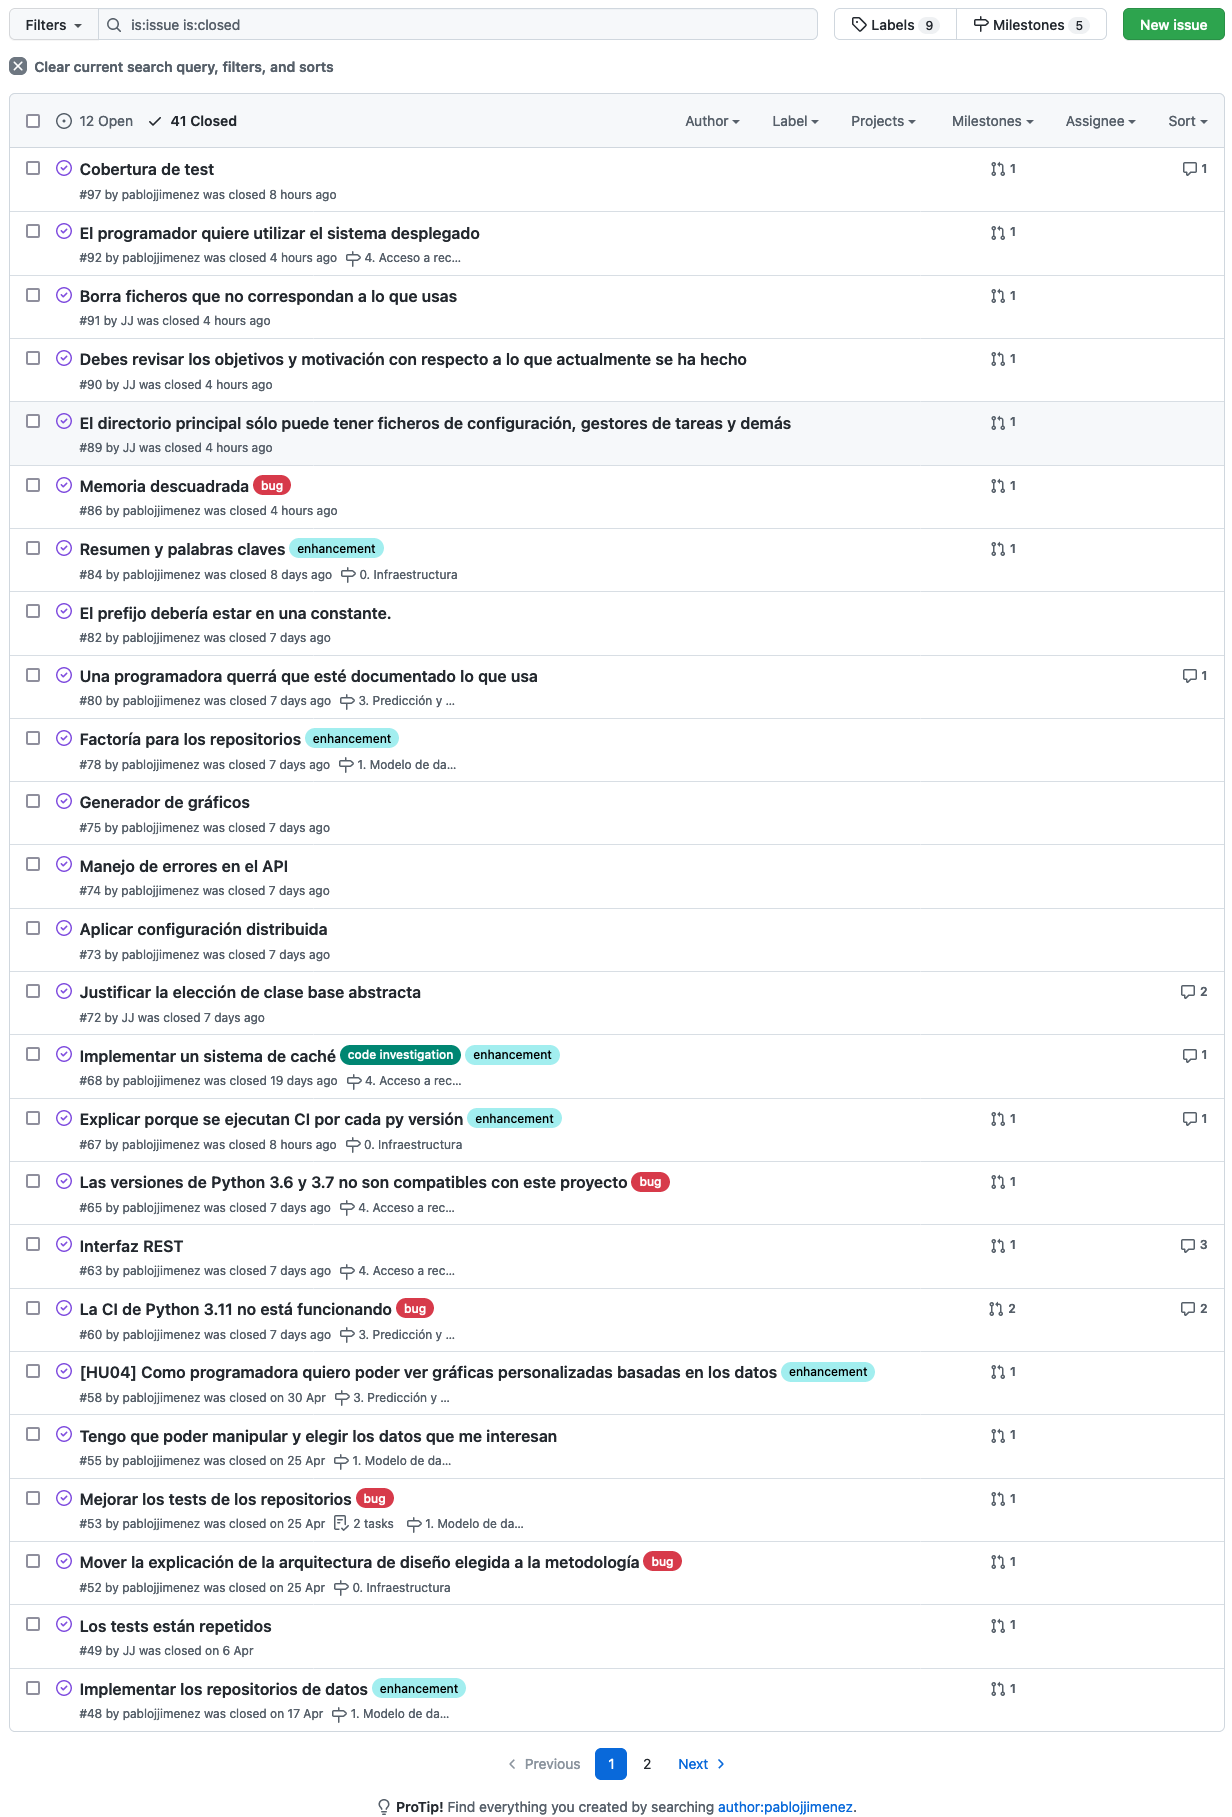
\includegraphics[width=\textwidth]{doc/logos/imgs/issues.png}
	\caption{ Issues del TFG vistas desde GitHub. }
    \label{fig:issues-HU}
\end{figure}
\FloatBarrier


\subsection{Integración continua}
\label{sec:ci}
Una buena forma de seguir cumpliendo con las características \hyperref[sec:meto]{citadas
anteriormente}, a nivel de transparencia y adaptación es adecuado realizar el
desarrollo guiado por pruebas, lo que se conoce por TDD, \textit{Test Driven Development}.
Al emplear esta metodología garantizamos la calidad de lo programado, trasladamos los
requisitos a las pruebas de forma que se convierten en la más fiable documentación. Además
tener una gran cobertura de código testeado nos permite poder refactorizar con asiduedad y
garantizarnos no generar deuda técnica. 

La integración continua o CI \textit{continuos integration} es uno de los pilares de la
filosofía DevOps, se basa en realizar integraciones frecuentes con la máxima seguridad
posible ya que garantizan que el sistema se proteja siempre al incluir nuevos cambios ya
que estos deben de superar las \textit{pipelines} para terminar integrándose. 

Desde el inicio del trabajo se ha estado trabajando con un sistema férreo de CI de forma
que no se ha mezclado nunca nada que no haya superado los requisitos de diseño
especificados. La tecnología utilizada ha sido \textit{Github Actions} que es
una herramienta de CI que nos permite realizar una integración continua de la misma forma
que \textit{Travis CI} la elección de Github sobre Travis es por la rapidez del elegido e
integración con la forja utilizada que como se ha especificado anteriormente es Github.

Para garantizar la \textbf{calidad de la memoria} se han implementado dos tipos de CI\: un
revisor ortográfico y un revisor de estructura que compila el documento automáticamente y
pública el PDF generado en las
\href{https://github.com/pablojjimenez/TFG/releases}{\textit{releases} del repositorio.}

Del mismo modo, para el \textbf{código} se han implementado otras dos CI que garantizan
que cuando se introduce en la rama principal del repositorio código nuevo, éste garantiza
unos estándares de calidad y que efectivamente el código es funcional por todas las
versiones especificadas de Python. Por un lado, para ausentar de errores el código fuente
y para comprobar la complejidad ciclomática. \footnote{Se ha utilizado la tecnología
\textbf{Flake8} por ser las más utilizada en el ecosistema. Algunos mensajes de error
pueden ser del tipo: \textit{library imported but unused} y \textit{Undefined name} } 

Por otro lado, se corre la \textit{suit} de tests de forma que se garantice que al añadir
uno código no se rompe el existente. 

\FloatBarrier
\begin{figure}[h]
	\centering	
	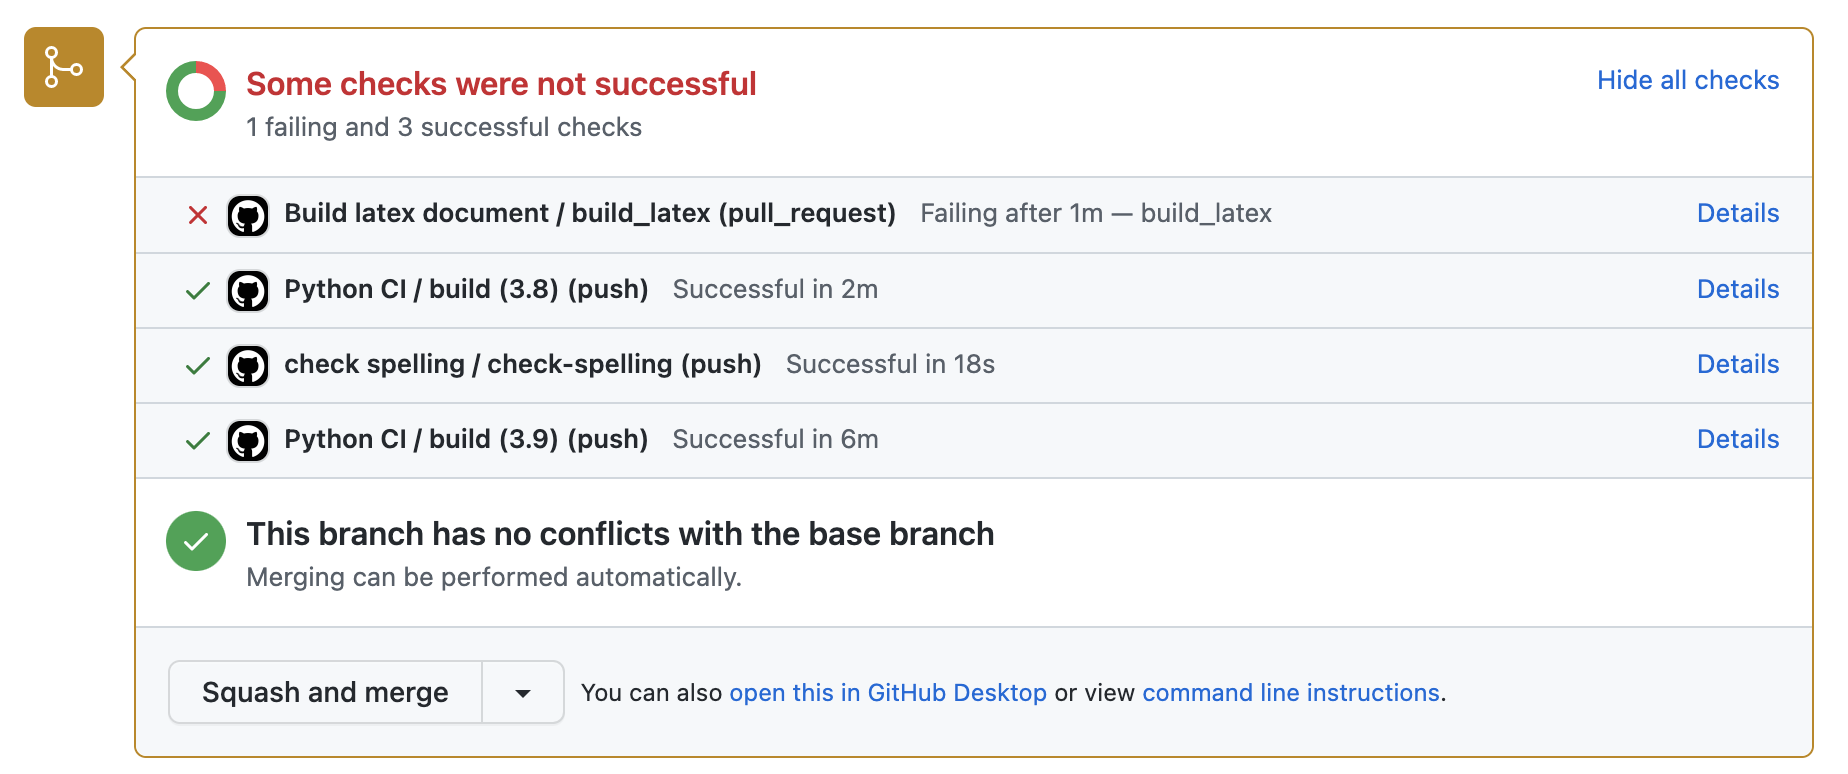
\includegraphics[width=\textwidth]{doc/logos/imgs/CI-pr.png}
    \caption{Ejemplo de ejecución automática de la CI}
    \label{fig:tipos-de-cc}
\end{figure}
\FloatBarrier


\section{Planificación y cuantificación}
La planificación temporal realizada ha sido la siguiente.

\renewcommand{\arraystretch}{1.5}
\begin{table}[H]
	\centering
	\resizebox{\textwidth}{!}{%
	\begin{tabular}{@{}ccc@{}}
		\toprule
		\rowcolor[HTML]{ECF4FF} 
		\textbf{Productos mínimos viables} & \textbf{Fecha de comienzo} & \textbf{Fecha de finalización} \\ \midrule
	    \textbf{1. Infraestructura} & 14 de marzo & 28 de marzo \\
	    \textbf{2. Modelo de datos} & 29 de abril & 2 de mayo \\
	    \textbf{3. Predicciones y gráficos} & 4 de mayo & 15 de mayo \\
	    \textbf{4. Acceso a recursos y managers} & 17 de mayo & 5 de junio \\
	    \textbf{5. Sistema avanzado de consultas} & 6 de junio & 26 de junio \\
		\textbf{6. Despliegue y entrega} & 27 de junio & 8 de julio \\ \bottomrule
	\end{tabular}}
	\caption{Organización temporal del proyecto.}
\end{table}

Durante el trabajo se ha ido anotando las horas dedicadas a cada uno de los milestones. En
el gráfico se añade también la última etapa de despliegue de la aplicación y trabajo final
antes de la entrega.

\FloatBarrier
\begin{figure}[h]
	\centering	
	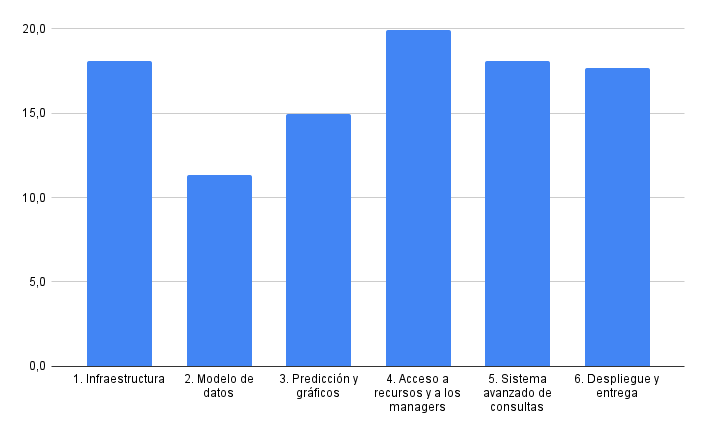
\includegraphics[width=\textwidth]{doc/logos/imgs/horas.png}
    \caption{Porcentaje de tiempo dedicado a las distintas etapas.}
    \label{fig:tipos-de-cc}
\end{figure}
\FloatBarrier

\subsection{Estimación de costes}
Es esta última sección vamos a detallar los costes asociados que tendría la elaboración
del proyecto.

\begin{table}[H]
\centering
    \begin{center}
        \begin{tabular}{| p{0.3\linewidth} | p{0.2\linewidth} | p{0.35\linewidth}|}
            \hline
            \rowcolor[HTML]{ECF4FF} 
            \textbf{Concepto} & \textbf{Coste} & \textbf{Comentarios} \\ \hline
            \textbf{MacBook Pro 2018} & 150 €/año & La cantidad de amortización aplicable es del 26\% a
        10 años. Con coste de compra: 1500€ \\
        \textbf{Recursos software} & 0 € &  \\
        \textbf{Recursos para el despliegue } & 23,94 €/mes & Puede consultarse en mayor
        detalle en \hyperref[sec:despliegue]{el capítulo 5, sección sobre el coste.}  \\
        \hline
        \end{tabular}
        \caption{Presupuesto del proyecto}
    \end{center}
\end{table}
